% Koma class
\documentclass[a4paper, oneside]{scrartcl}   

\usepackage{a4wide}

%------------------
% language = english
\usepackage[english, german]{babel}	% Umlaute mit \"u
\usepackage[latin1]{inputenc}
\usepackage{enumitem}

% margins + Kopf- und Fusszeilen
\usepackage[left = 2.5cm, right = 2.5cm, top = 2cm, bottom = 3cm]{geometry}
\usepackage{scrpage2} 
\pagestyle{scrheadings}
\clearscrheadfoot
\rehead{\headmark}
\lehead{\pagemark}
\lohead{\headmark}
\rohead{\pagemark} 

% math
\usepackage{amssymb}
\usepackage{amsmath}

% figures
\usepackage{tikz}
\usepackage{graphicx}

% section-Zaehler wird neu gesetzt:
\setcounter{section}{11}
%------------------
\author{Sascha Meiers, Martin Seeger}
\title{Exercise 11, Discrete Mathematics for Bioinformatics}
\date{Winter term 2011/2012}


\begin{document}
\maketitle

%---------------------------------------------------------------------------------------------------

\subsection{Lagrangean Relaxation I}

\renewcommand{\labelenumi}{\alph{enumi})}
\begin{enumerate}
  \item Polytope for original problem:\\
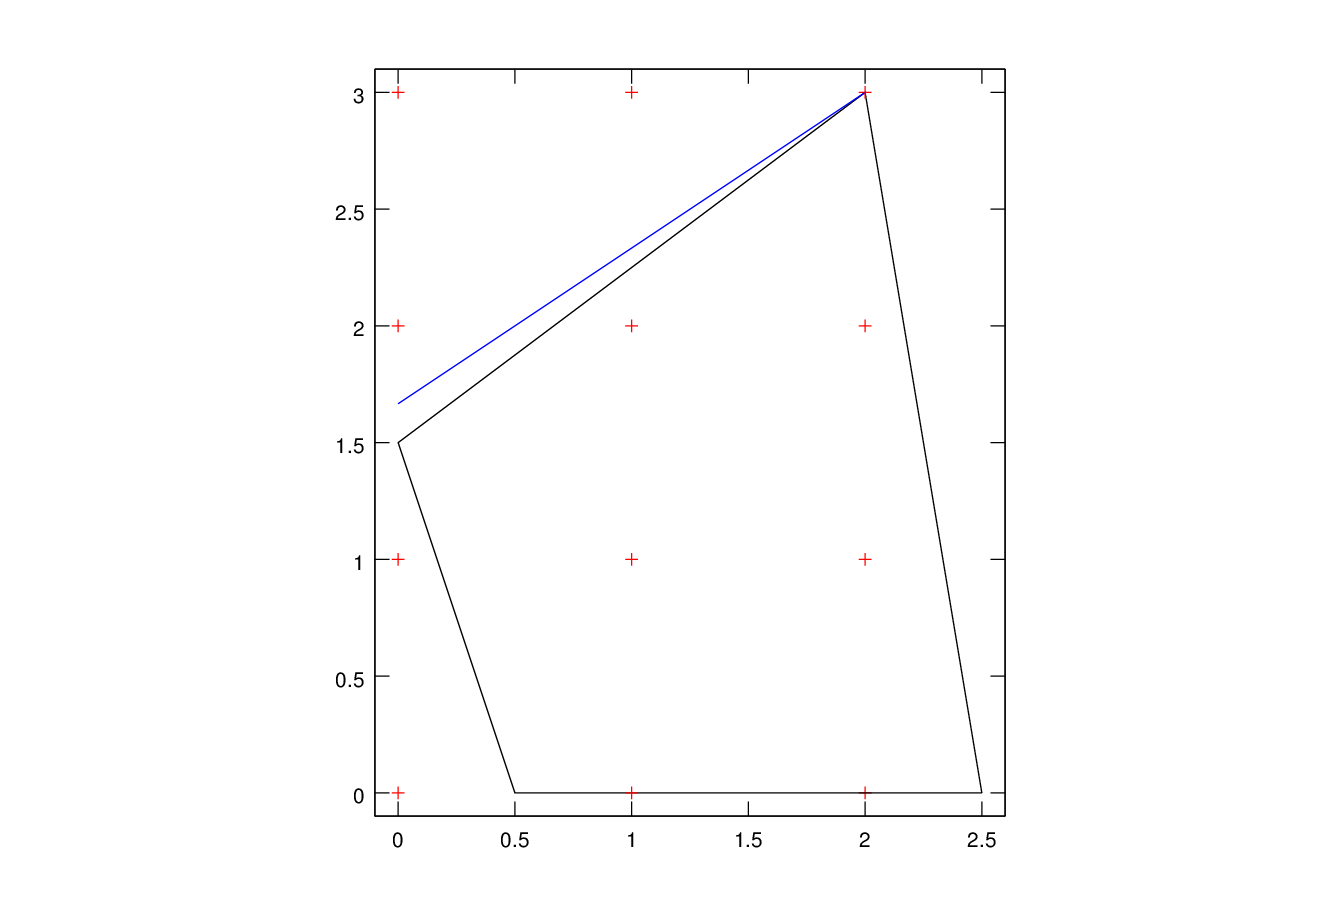
\includegraphics[width=\textwidth]{ex11_1_a_good.png}
The optimal value is reached at $(x_1, x_2)=(2, 3)$ with $Z_{IP}=Z_{LP}=-5$.
  \item Polytope for relaxed problem:\\
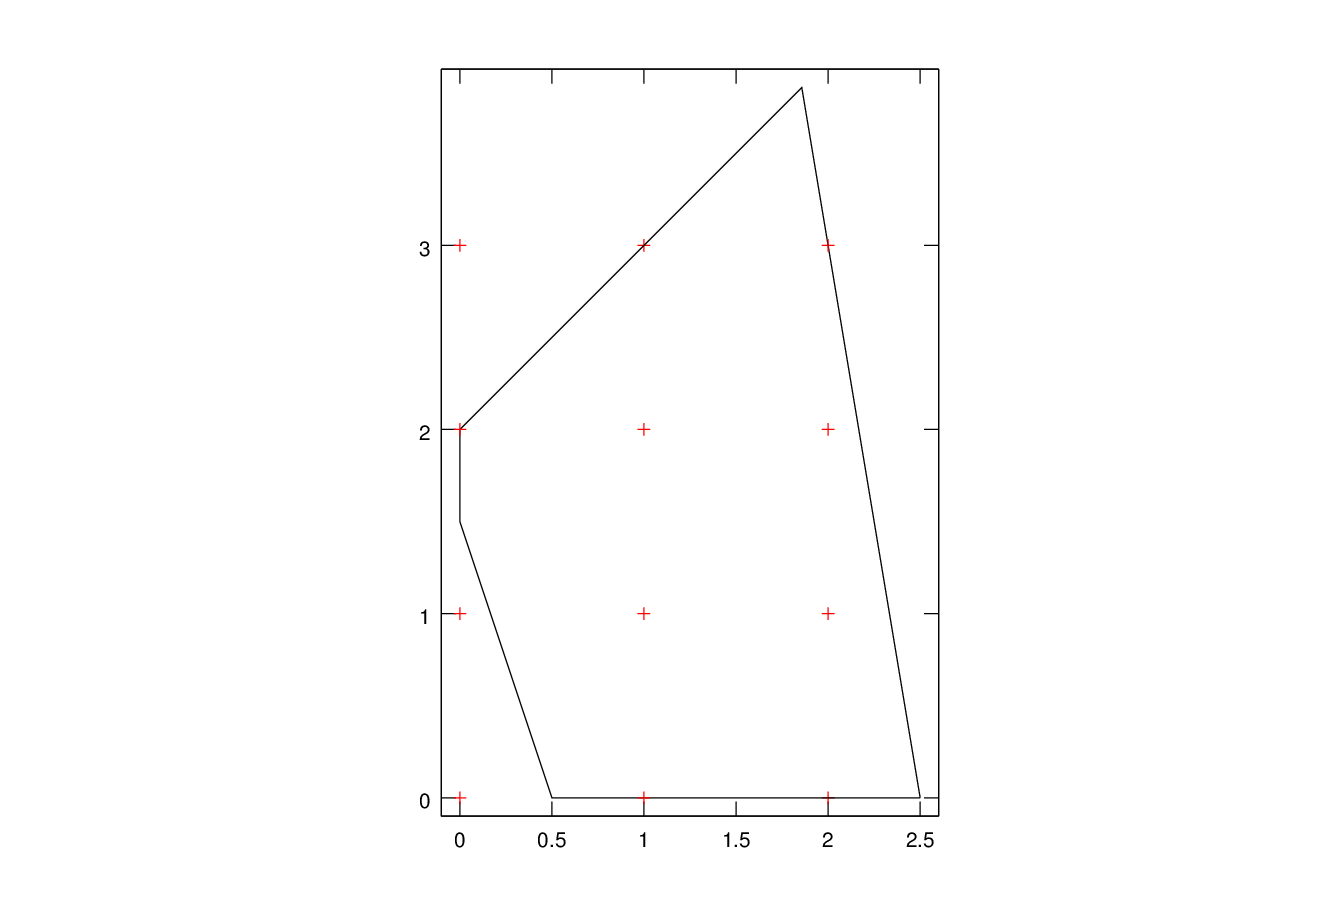
\includegraphics[width=\textwidth]{ex11_1_b_good.png}\\
Set of feasible solutions for this problem: 
\[
X = \{(1, 0), (2, 0), (1, 1), (2,
1), (0, 2), (1, 2), (2, 2), (1, 3), (2, 3)\}.
\]
\item With the Lagrange multiplier, $Z_D =$ maximum of the minima. This can be
read off the following chart:\\
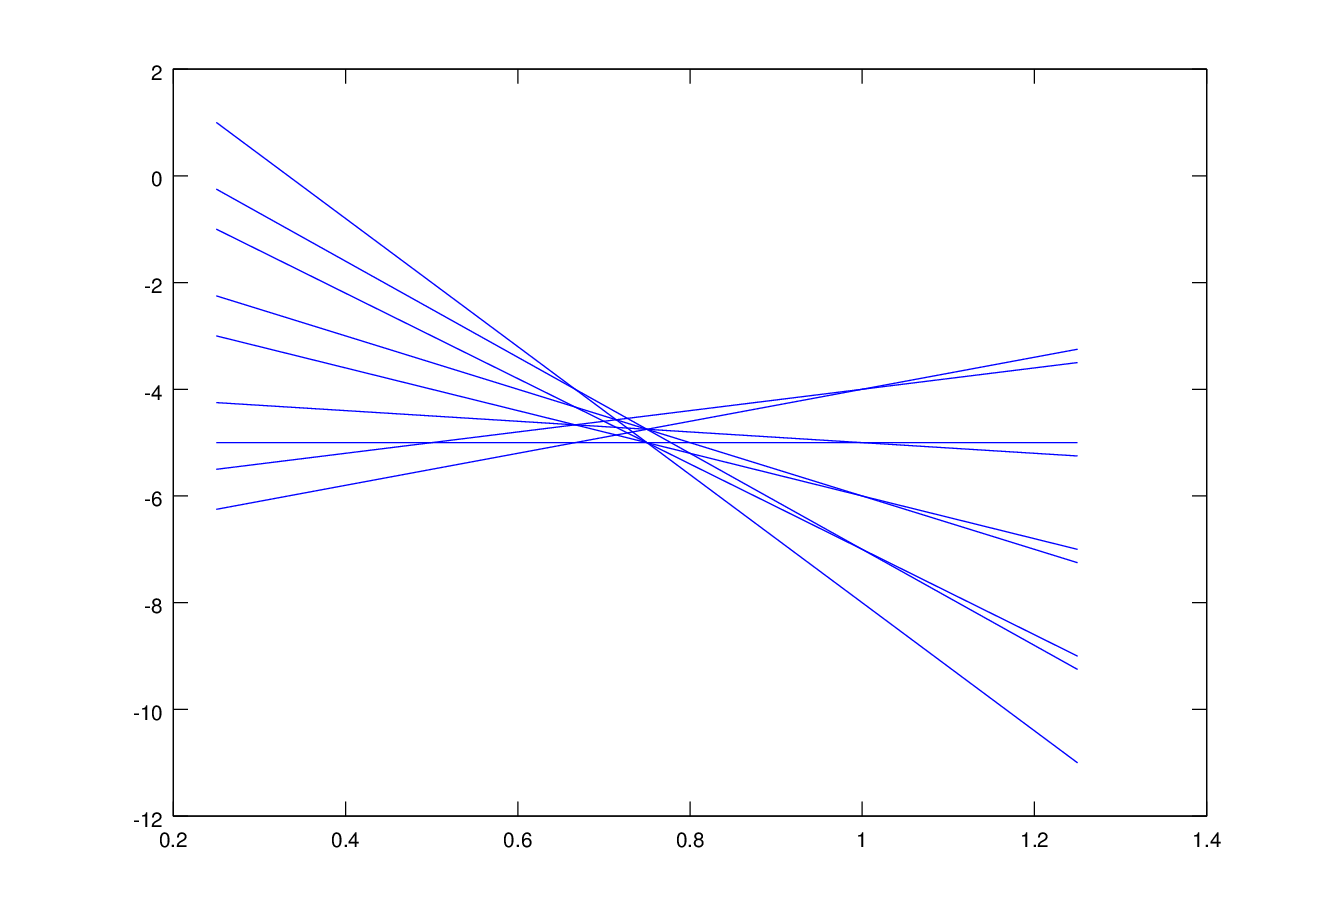
\includegraphics[width=\textwidth]{ex11_1_c_good.png}\\
We find that $Z_D = Z_{IP} = Z_{LP} = -5$.
\end{enumerate}

\subsection{Lagrangean Relaxation II}

We have 
\begin{align}
Z_{IP} &= \text{min } \{ c^T x \; | \; Ax \geq b, \; Dx \geq d\} \\
Z(\lambda) &= \text{min } \{ c^T x + \lambda^T (b-Ax) \; | \; Dx \geq d\}
\end{align}
and can derive
\[ Z_{IP} \geq \text{min } \{ c^T x + \lambda^T (b-Ax) \; | \; Ax \geq b, \; Dx \geq d\} =: Z_{+} \]
because
\[b-Ax \leq 0  \text{ and } \lambda \geq 0. \]
Finally we have 
\[Z_{+} \geq Z(\lambda) \]
since 
\[ \{x \; | \; Ax\geq b, \; Dx \geq d\} \subseteq \{x \; | \; Dx\geq d\} \]

\subsection{Structural alignment}

\noindent \textbf{Proof: The polytope is full-dimensional}

The matrix below shows $n+m$ linearly independent column vectors, each one representing a feasible solution.
\[
\begin{array}{c|cccc|cccc}
e_1    & 1       & 0 & \hdots & 0      &   &   &        &   \\
e_2    & 0       & 1 &        & 0      &   & A &        &   \\
\vdots & \vdots  &   & \ddots &        &   &   &        &   \\
e_n    & 0       & 0 &        & 1      &   &   &        &   \\ 
\hline
i_1    & 0       & 0 & \hdots & 0      & 1 & 0 & \hdots & 0 \\
i_2    & 0       & 0 &        & 0      & 0 & 1 &        & 0 \\
\vdots & \vdots  &   & \ddots &        &   &   & \ddots &   \\
i_m    & 0       & 0 &        & 0      & 0 & 0 &        & 1 \\
\end{array}
\]
where in $A$ every column contains two $1$ values at $e_l$ and $e_r$, 
corresponding to the two alignment edges that enable the interaction match $i_j = (l,r)$.

Since these vectors are linearly independent, they're affinely independent, too.

\vspace{5mm} \noindent \textbf{Proof: $x_i \leq 1$ is facet-defining}

$\Rightarrow$ By setting the complete row $e_i$ to value $1$, we satisfy the constraint $x_i \leq 1$ with equality.
This only leads to feasible solutions, if $e_i$ is not in conflict with another edge $e_j$. 
These columns are still linearly independent.

$\Leftarrow$ We are given $n+m$ affinely independent vectors with $e_i=1$ that prove the facet-property of $x_i \leq 1$.
Now we assume that there is an edge $e_j, j\neq i$ that is in conflict with $e_i$. This means, in all $n+m$ 
vectors the $e_j$ entry must be zero. These vectors are no longer affinely independent, as we will see:

Let $k = m+n$. The vectors $v_1, ..., v_k$ are affinely independent, if and only if the vectors 
$v_2-v_1, ..., v_k-v_1$ are linearly independent. These are $k-1$ vecors, but all of them have value zero in position $e_i$ and $e_j$!
Obviously $k-1$ vectors with only $k-2$ rows cannot be linearly independent!

\vspace{5mm} \noindent \textbf{Proof: $x_i \geq 0$ is facet-defining}

?


\end{document}
